% Architecture 3 (M13) --- detailed diagrams and novelty summary.
% Canonical copy lives in docs3/ (companion markdown specs in the same folder).
% Landscape A4, same visual language as docs2/proposed_architecture_landscape.tex
% and docs1/pipeline_diagrams_landscape.tex.
% Compile with:  cd docs3 && tectonic arch3_architecture_landscape.tex
%                (or pdflatex twice)
%
% Status: correctness checks passed in M13 (M13 CHECKS OK, arch3_spec.json).
% Pilot training not yet run. Arch 2 (SB-LN + LN-value offsets) remains scratched.
\documentclass[11pt]{article}
\usepackage[a4paper,landscape,margin=14mm]{geometry}
\usepackage{lmodern}
\usepackage{amsmath,amssymb}
\usepackage{xcolor}
\usepackage{array,booktabs}
\usepackage{tikz}
\usetikzlibrary{arrows.meta,positioning,fit,backgrounds,calc}
\pagestyle{empty}
\setlength{\parindent}{0pt}
\newcolumntype{L}[1]{>{\raggedright\arraybackslash}p{#1}}

\definecolor{box}{HTML}{EEF2F7}
\definecolor{trn}{HTML}{FCE9C8}
\definecolor{frz}{HTML}{DCE6F2}
\definecolor{prv}{HTML}{E3F1DF}
\definecolor{nov}{HTML}{F8E6EF}   % novelty callout

\tikzset{
  blk/.style={draw,rounded corners=3pt,fill=box,align=center,font=\normalsize,minimum height=19mm,text width=46mm,line width=0.8pt},
  frz/.style={blk,fill=frz},
  trn/.style={blk,fill=trn},
  prv/.style={blk,fill=prv},
  nov/.style={blk,fill=nov},
  lab/.style={font=\footnotesize,text=black!80,inner sep=1.5pt},
  ar/.style={-{Latex[length=3mm]},line width=1.1pt}}

\newcommand{\sg}{\operatorname{sg}}

\begin{document}

% =====================================================================
% PAGE 1: inference pipeline
% =====================================================================
\begin{center}
{\Large\bfseries Architecture 3 --- Inference Pipeline}\\[2pt]
{\small Orange = trained \& deployed (34{,}370 at \(r{=}16\)); green = training-only (discarded); blue = frozen CLIP; grey = fixed / buffer.
Private \(\delta_g\) is \textbf{not} used at inference (\(\delta{=}0\)).}
\end{center}
\vspace{3mm}

\begin{center}
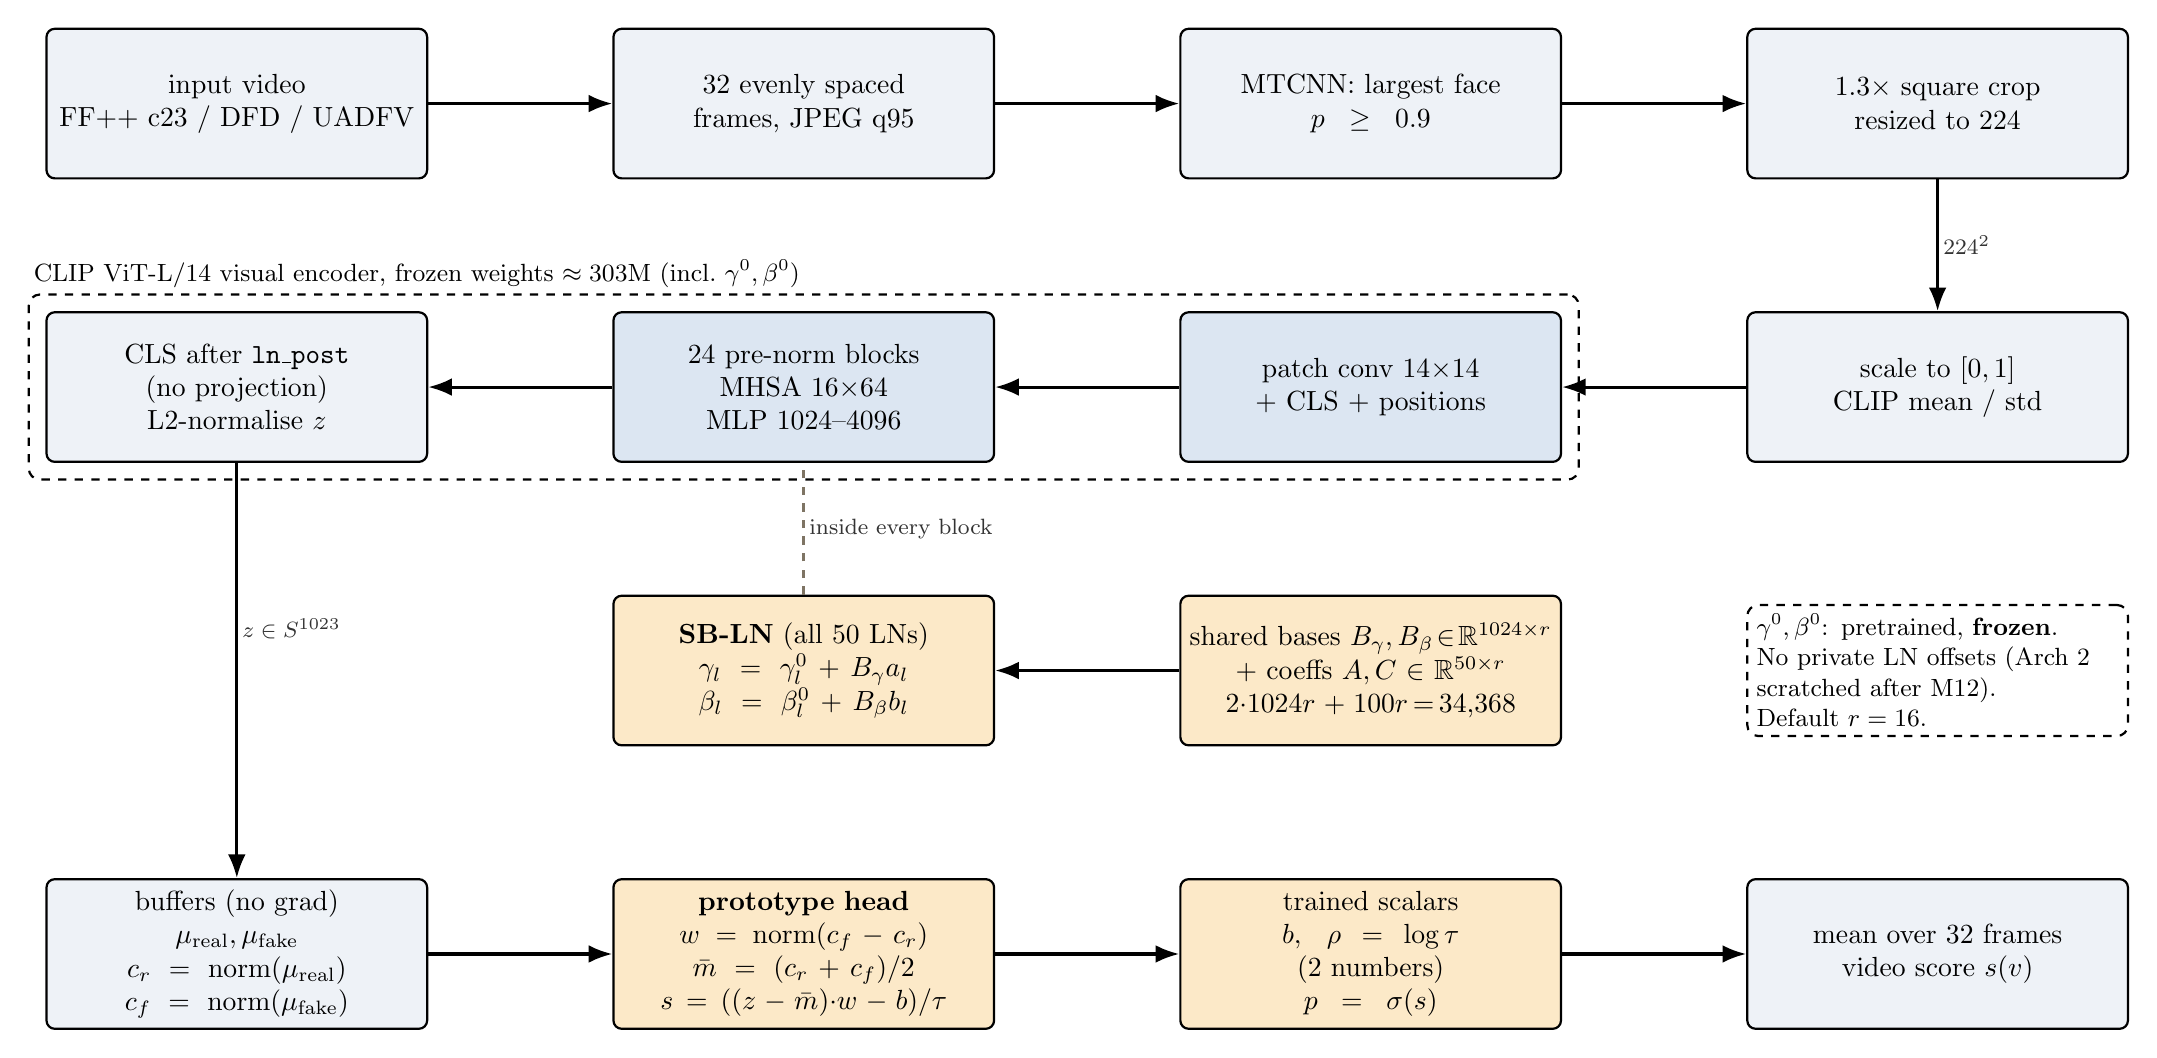
\begin{tikzpicture}[x=72mm,y=-36mm]
% row 0: preprocess (unchanged from Arch 1 / M4)
\node[blk] (vid) at (0,0) {input video\\FF++ c23 / DFD / UADFV};
\node[blk] (frm) at (1,0) {32 evenly spaced\\frames, JPEG q95};
\node[blk] (det) at (2,0) {MTCNN: largest face\\\(p\ge0.9\)};
\node[blk] (crp) at (3,0) {1.3\(\times\) square crop\\resized to 224};
% row 1: encoder
\node[blk] (pre) at (3,1) {scale to \([0,1]\)\\CLIP mean / std};
\node[frz] (pe)  at (2,1) {patch conv 14\(\times\)14\\+ CLS + positions};
\node[frz] (tr)  at (1,1) {24 pre-norm blocks\\MHSA 16\(\times\)64\\MLP 1024--4096};
\node[blk] (cls) at (0,1) {CLS after \texttt{ln\_post}\\(no projection)\\L2-normalise \(z\)};
% row 2: SB-LN (novelty N1, shared)
\node[trn] (sbln) at (1,2) {\textbf{SB-LN} (all 50 LNs)\\\(\gamma_l=\gamma_l^0+B_\gamma a_l\)\\\(\beta_l=\beta_l^0+B_\beta b_l\)};
\node[trn] (sbp)  at (2,2) {shared bases \(B_\gamma,B_\beta\!\in\!\mathbb{R}^{1024\times r}\)\\+ coeffs \(A,C\!\in\!\mathbb{R}^{50\times r}\)\\\(2{\cdot}1024r+100r\)\,=\,34{,}368};
\node[draw,dashed,rounded corners,font=\small,align=left,text width=46mm,line width=0.8pt] (nt) at (3,2)
 {\(\gamma^0,\beta^0\): pretrained, \textbf{frozen}.\\No private LN offsets (Arch~2 scratched after M12).\\Default \(r=16\).};
% row 3: prototype head at δ=0
\node[blk] (buf) at (0,3) {buffers (no grad)\\\(\mu_\text{real},\mu_\text{fake}\)\\\(c_r=\mathrm{norm}(\mu_\text{real})\)\\\(c_f=\mathrm{norm}(\mu_\text{fake})\)};
\node[trn] (hd)  at (1,3) {\textbf{prototype head}\\\(w=\mathrm{norm}(c_f-c_r)\)\\ \(\bar m=(c_r+c_f)/2\)\\ \(s=((z-\bar m){\cdot}w-b)/\tau\)};
\node[trn] (par) at (2,3) {trained scalars\\\(b,\;\rho=\log\tau\)\\(2 numbers)\\ \(p=\sigma(s)\)};
\node[blk] (agg) at (3,3) {mean over 32 frames\\video score \(s(v)\)};
% arrows
\draw[ar] (vid)--(frm); \draw[ar] (frm)--(det); \draw[ar] (det)--(crp);
\draw[ar] (crp)--node[lab,right]{\(224^2\)}(pre);
\draw[ar] (pre)--(pe); \draw[ar] (pe)--(tr); \draw[ar] (tr)--(cls);
\draw[ar] (cls)--node[lab,right,pos=0.4]{\(z\in S^{1023}\)}(buf);
\draw[ar] (buf)--(hd); \draw[ar] (hd)--(par); \draw[ar] (par)--(agg);
\draw[ar] (sbp)--(sbln);
\draw[line width=1.1pt,dashed,trn!50!black] (sbln)--node[lab,right]{inside every block}(tr);
\begin{scope}[on background layer]
\node[draw,dashed,rounded corners,fit=(pe)(tr)(cls),inner sep=6pt,line width=0.8pt] (bb) {};
\end{scope}
\node[font=\small,anchor=south west,inner sep=2pt] at (bb.north west)
 {CLIP ViT-L/14 visual encoder, frozen weights \(\approx303\)M (incl.\ \(\gamma^0,\beta^0\))};
\end{tikzpicture}
\end{center}

\vfill
{\small\textbf{Deployed vs.\ Arch~1:} 104{,}450 (50 LNs + linear head) \(\to\) 34{,}370 (SB-LN \(r{=}16\) + prototype). Linear head \(1024{\to}2\) is \textbf{not} used. Training-only private latent \(\delta_g\) (next pages) is discarded here --- same deploy pattern as GBLA, but \(\delta\) never lived on LayerNorm values.}

\newpage
% =====================================================================
% PAGE 2: private feature latent (the Arch 3 novelty vs Arch 2)
% =====================================================================
\begin{center}
{\Large\bfseries Novelty: Feature-Space Private Latent \(\delta_g\) (Training Only)}\\[2pt]
{\small Not GBLA / Arch~2 LN-value offsets. \(\delta_g\) shifts the \textbf{fake centroid in feature space}; the new loss term is defined through that centroid.}
\end{center}
\vspace{2mm}

\begin{center}
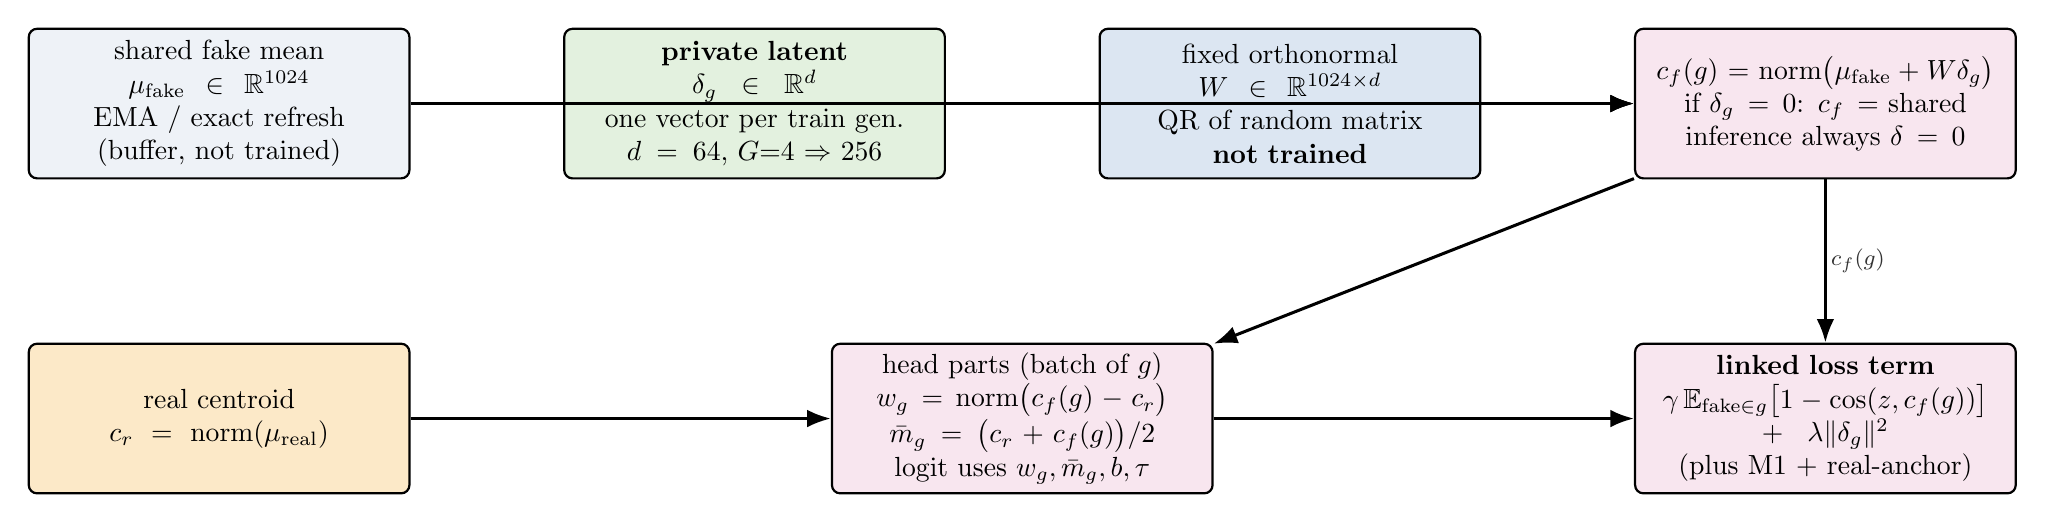
\begin{tikzpicture}[x=68mm,y=-40mm]
\node[blk] (mu) at (0,0) {shared fake mean\\\(\mu_\text{fake}\in\mathbb{R}^{1024}\)\\EMA / exact refresh\\(buffer, not trained)};
\node[prv] (dlt) at (1,0) {\textbf{private latent}\\\(\delta_g\in\mathbb{R}^{d}\)\\one vector per train gen.\\ \(d=64\), \(G{=}4\) \(\Rightarrow\) 256};
\node[frz] (W) at (2,0) {fixed orthonormal\\ \(W\in\mathbb{R}^{1024\times d}\)\\QR of random matrix\\ \textbf{not trained}};
\node[nov] (cf) at (3,0) {\(c_f(g)=\mathrm{norm}\big(\mu_\text{fake}+W\delta_g\big)\)\\if \(\delta_g=0\): \(c_f=\) shared\\inference always \(\delta=0\)};

\node[trn] (cr) at (0,1) {real centroid\\\(c_r=\mathrm{norm}(\mu_\text{real})\)};
\node[nov] (hp) at (1.5,1) {head parts (batch of \(g\))\\ \(w_g=\mathrm{norm}\big(c_f(g)-c_r\big)\)\\ \(\bar m_g=\big(c_r+c_f(g)\big)/2\)\\logit uses \(w_g,\bar m_g,b,\tau\)};
\node[nov] (loss) at (3,1) {\textbf{linked loss term}\\\(\gamma\,\mathbb{E}_{\text{fake}\in g}\big[1-\cos(z,c_f(g))\big]\)\\ \(+\;\lambda\|\delta_g\|^2\)\\(plus M1 + real-anchor)};

\draw[ar] (mu)--(cf); \draw[ar] (dlt)--(cf); \draw[ar] (W)--(cf);
\draw[ar] (cr)--(hp); \draw[ar] (cf)--(hp); \draw[ar] (hp)--(loss);
\draw[ar] (cf)--node[lab,right]{\(c_f(g)\)}(loss);
\end{tikzpicture}
\end{center}

\vspace{4mm}
\begin{center}
\small
\begin{tabular}{L{48mm}L{55mm}L{55mm}L{55mm}}
\toprule
 & \textbf{Arch 1 (GBLA)} & \textbf{Arch 2 (scratched)} & \textbf{Arch 3 (this)} \\
\midrule
Shared adapter & 50 full LNs & SB-LN & SB-LN (\(r{=}16\)) \\
Head & linear 2{,}050 & linear / prototype & prototype (\(b,\tau\)) \\
Private latent & \(\delta_g\) on LN \(\gamma,\beta\) & \(\delta_g\) on LN under SB-LN & \(\delta_g\) in \textbf{feature} space \\
Loss \(\leftrightarrow\) private & \(\lambda\|\delta\|^2\) (+ optional \(w_g\)) & \(w_g{\cdot}\)CE failed (M12) & \(\gamma\)-attract to \(c_f(\delta)\) \(+\,\lambda\|\delta\|^2\) \\
Deployed \(P\) & 104{,}450 & \(\sim\)34k--36k & \textbf{34{,}370} \\
Train-time extra & \(G{\times}104{,}450\) & \(G{\times}2{\times}50{\times}1024\) & \(G{\times}d=256\) \\
\bottomrule
\end{tabular}
\end{center}

\vfill
{\small\textbf{Why not Arch~2 again.} M12: private LN offsets under SB-LN hurt NeuralTextures (A2 \(\Delta\)NT \(=-2.5\); A3 \(w_g{\cdot}\)CE \(\Delta\)NT \(=-18.6\)). Arch~3 keeps compression (SB-LN) but moves the private latent off LayerNorms and wires it only through \(c_f(g)\) and the attraction term.}

\newpage
% =====================================================================
% PAGE 3: training workflow + full loss
% =====================================================================
\begin{center}
{\Large\bfseries Architecture 3 --- Training Workflow and Full Loss}\\[2pt]
{\small Same data order / schedule as M4 (round-robin pure-generator blocks, 10 epochs, seed 0). \(\delta_g\) is active only while training generator \(g\).}
\end{center}
\vspace{4mm}

\begin{center}
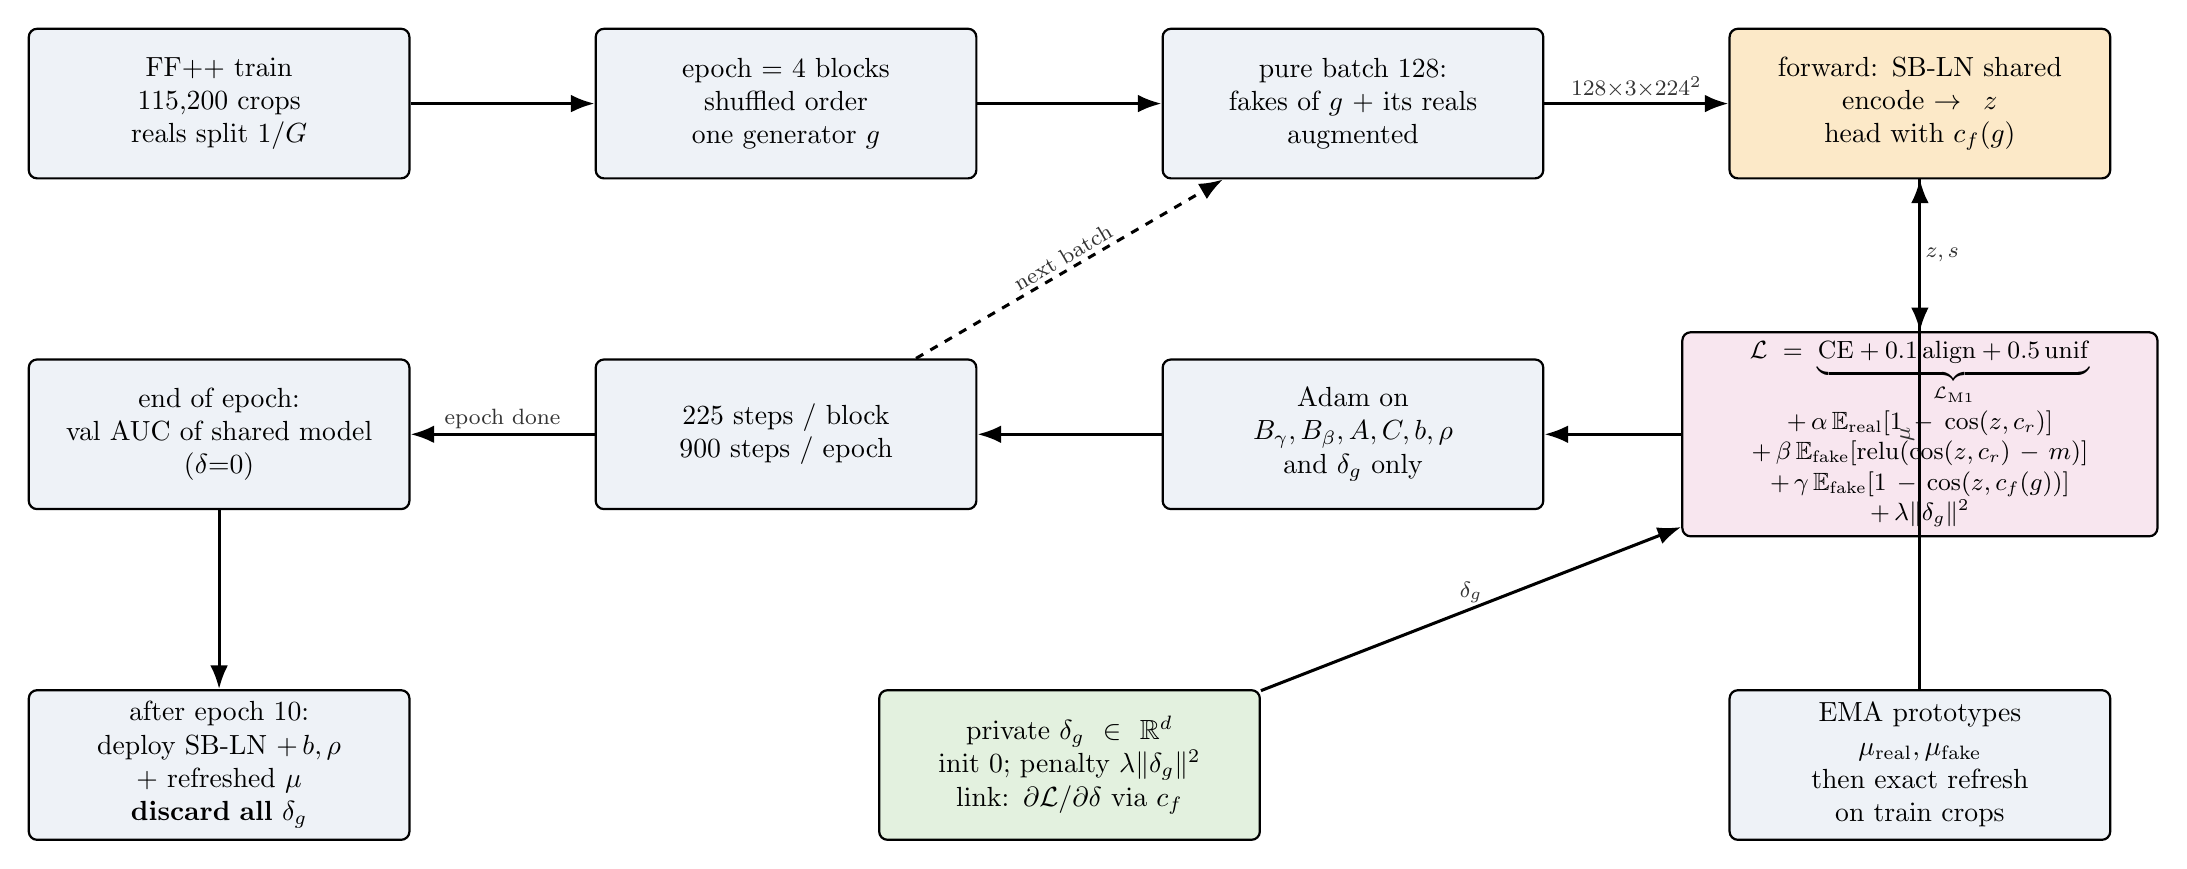
\begin{tikzpicture}[x=72mm,y=-42mm]
\node[blk] (ds)  at (0,0) {FF++ train\\115{,}200 crops\\reals split \(1/G\)};
\node[blk] (blk) at (1,0) {epoch = 4 blocks\\shuffled order\\one generator \(g\)};
\node[blk] (bat) at (2,0) {pure batch 128:\\fakes of \(g\) + its reals\\augmented};
\node[trn] (fw)  at (3,0) {forward: SB-LN shared\\encode \(\to z\)\\head with \(c_f(g)\)};
\node[nov,text width=58mm,font=\small] (L) at (3,1)
 {\(\mathcal{L}=\underbrace{\mathrm{CE}+0.1\,\mathrm{align}+0.5\,\mathrm{unif}}_{\mathcal{L}_{\mathrm{M1}}}\)\\[1pt]
  \(+\,\alpha\,\mathbb{E}_{\mathrm{real}}[1-\cos(z,c_r)]\)\\
  \(+\,\beta\,\mathbb{E}_{\mathrm{fake}}[\mathrm{relu}(\cos(z,c_r)-m)]\)\\
  \(+\,\gamma\,\mathbb{E}_{\mathrm{fake}}[1-\cos(z,c_f(g))]\)\\
  \(+\,\lambda\|\delta_g\|^2\)};
\node[blk] (bp)  at (2,1) {Adam on\\\(B_\gamma,B_\beta,A,C,b,\rho\)\\and \(\delta_g\) only};
\node[blk] (nxt) at (1,1) {225 steps / block\\900 steps / epoch};
\node[blk] (val) at (0,1) {end of epoch:\\val AUC of shared model\\(\(\delta{=}0\))};
\node[blk] (fin) at (0,2) {after epoch 10:\\deploy SB-LN \(+\,b,\rho\)\\+ refreshed \(\mu\)\\ \textbf{discard all \(\delta_g\)}};
\node[prv] (dlt) at (1.5,2) {private \(\delta_g\in\mathbb{R}^{d}\)\\init 0; penalty \(\lambda\|\delta_g\|^2\)\\link: \(\partial\mathcal{L}/\partial\delta\) via \(c_f\)};
\node[blk] (ema) at (3,2) {EMA prototypes\\\(\mu_\text{real},\mu_\text{fake}\)\\then exact refresh\\on train crops};
\draw[ar] (ds)--(blk); \draw[ar] (blk)--(bat);
\draw[ar] (bat)--node[lab,above]{\(128{\times}3{\times}224^2\)}(fw);
\draw[ar] (fw)--node[lab,right]{\(z,s\)}(L);
\draw[ar] (L)--(bp); \draw[ar] (bp)--(nxt);
\draw[ar,dashed] (nxt)--node[lab,above,sloped]{next batch}(bat);
\draw[ar] (nxt)--node[lab,above]{epoch done}(val);
\draw[ar] (val)--(fin);
\draw[ar] (dlt)--node[lab,above]{\(\delta_g\)}(L);
\draw[ar] (ema)--node[lab,above,sloped]{\(\mu\)}(fw);
\end{tikzpicture}
\end{center}

\vspace{3mm}
\begin{center}
\small
\begin{tabular}{lrrrr}
\toprule
hyperparameter & symbol & default & selected on & notes \\
\midrule
SB-LN rank & \(r\) & 16 & fixed (M11a / M13) & same as A0 \\
private dim & \(d\) & 64 & fixed before train & \(W\) fixed orthonormal \\
LN penalty & \(\lambda\) & 0.01 & as M4/M11b & on \(\|\delta_g\|^2\) only \\
real pull & \(\alpha\) & 0.1 & fixed before train & \\
fake margin & \(\beta,m\) & 1.0,\;0.1 & fixed before train & off \(c_r\) \\
attract to \(c_f(\delta)\) & \(\gamma\) & 0.5 & fixed before train & \textbf{δ \(\leftrightarrow\) loss link} \\
M1 weights & & 0.1 / 0.5 & as M1 & align / uniform \\
schedule & & 10 ep, \(3{\cdot}10^{-4}{\to}10^{-5}\) & as M4 & seed 0 \\
\bottomrule
\end{tabular}
\end{center}

\vfill
{\small\textbf{Pilot decision rule (pre-registered):} keep Arch~3 only if NT \(\ge\) A0 (81.21) and DFD \(\ge95.5\); else negative result and Arch~1 remains the only main model. Nothing is tuned on test data.}

\newpage
% =====================================================================
% PAGE 4: parameter budget
% =====================================================================
\begin{center}
{\Large\bfseries Parameter Budget --- Arch 3 vs Arch 1 / Side Baselines}\\[2pt]
{\small Counts from M13 after checks. Frozen CLIP weights \(\approx303\)M are shared by all rows and omitted from ``trainable''.}
\end{center}
\vspace{6mm}

\begin{center}
\small
\renewcommand{\arraystretch}{1.2}
\begin{tabular}{L{62mm}rrrL{55mm}}
\toprule
model & adapter & head / other & \textbf{deployed} & comment \\
\midrule
Arch 1 --- GBLA \(\lambda{=}0.01\) (M4) & 102{,}400 LN & 2{,}050 linear & \textbf{104{,}450} & published main \\
Full LN \(\lambda{=}\infty\) (M4) & 102{,}400 LN & 2{,}050 linear & 104{,}450 & no private \\
A0 --- SB-LN \(r{=}16\) + linear (M11a) & 34{,}368 & 2{,}050 & 36{,}418 & SB-LN side result \\
M11b --- SB-LN + LN-\(\delta\) + GBRA + proto & 34{,}368 & 2 + LN-\(\delta\) train & 34{,}370 dep.\ & Arch~2 family; NT fell \\
\textbf{Arch 3 --- SB-LN + proto + feat-\(\delta\)} & 34{,}368 & 2 & \textbf{34{,}370} & \textbf{this work} \\
\midrule
Arch 3 train-time only (\(+\,G{\cdot}d\)) & & \(+256\) & 34{,}626 stored & discarded after train \\
Arch 2-style LN-\(\delta\) train-time (ref.) & & \(+G{\cdot}2{\cdot}50{\cdot}1024\) & \(+409{,}600\) & scratched (M12) \\
\bottomrule
\end{tabular}
\end{center}

\vspace{8mm}
\begin{center}
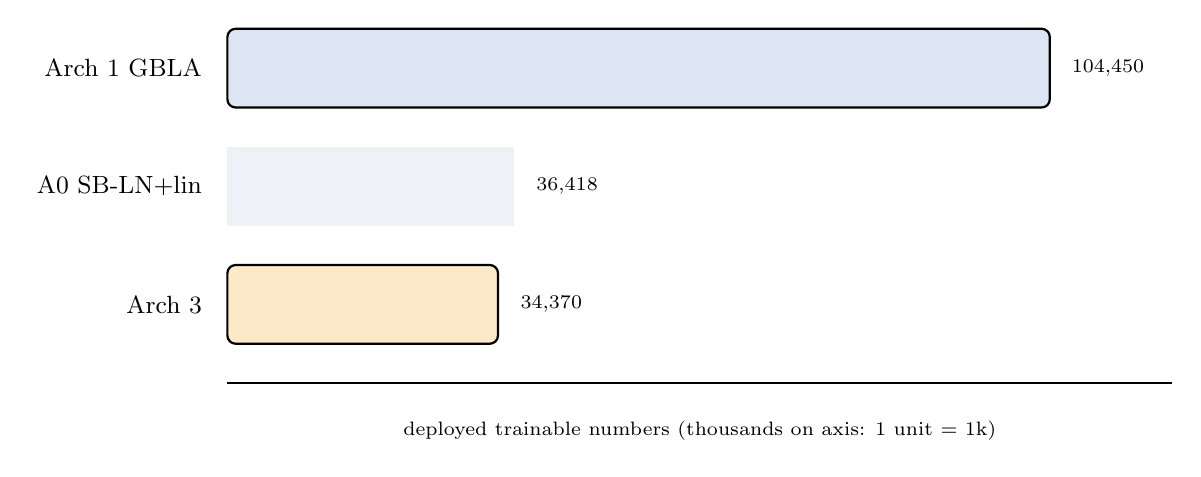
\begin{tikzpicture}[x=1mm,y=1mm]
% bar chart of deployed params
\node[font=\small,anchor=east] at (-2,40) {Arch 1 GBLA};
\node[font=\small,anchor=east] at (-2,25) {A0 SB-LN+lin};
\node[font=\small,anchor=east] at (-2,10) {Arch 3};
\fill[frz] (0,35) rectangle (104.45,45);
\fill[box] (0,20) rectangle (36.418,30);
\fill[trn] (0,5) rectangle (34.370,15);
\node[font=\scriptsize,anchor=west] at (106,40) {104{,}450};
\node[font=\scriptsize,anchor=west] at (38,25) {36{,}418};
\node[font=\scriptsize,anchor=west] at (36,10) {34{,}370};
\draw[line width=0.6pt] (0,0)--(120,0);
\node[font=\scriptsize] at (60,-6) {deployed trainable numbers (thousands on axis: 1 unit = 1k)};
\end{tikzpicture}
\end{center}

\vspace{6mm}
\begin{center}
\small
\begin{tabular}{L{70mm}rr}
\toprule
Arch 3 piece & count & deployed? \\
\midrule
SB-LN bases \(B_\gamma,B_\beta\) (\(2{\cdot}1024{\cdot}16\)) & 32{,}768 & yes \\
SB-LN coeffs \(A,C\) (\(2{\cdot}50{\cdot}16\)) & 1{,}600 & yes \\
prototype \(b,\rho\) & 2 & yes \\
\textbf{total deployed} & \textbf{34{,}370} & \\
\midrule
private \(\delta_g\) (\(4{\times}64\)) & 256 & no (train only) \\
projection \(W\) (fixed QR) & 0 trained & buffer \\
EMA / exact \(\mu_\text{real},\mu_\text{fake}\) & 0 trained & buffer \\
\textbf{total train-time} & \textbf{34{,}626} & \\
\bottomrule
\end{tabular}
\end{center}

\vfill
{\small Reduction vs.\ Arch~1 deployed: \(104{,}450/34{,}370\approx3.04\times\). Private train-time overhead: 256 vs.\ GBLA's \(4{\times}104{,}450\) or Arch~2's LN offsets.}

\newpage
% =====================================================================
% PAGE 5: novelty summary table
% =====================================================================
\begin{center}
{\Large\bfseries Architecture 3 --- Claimed Novelties}\\[2pt]
{\small Relative to Arch~1 (published GBLA) and the scratched Arch~2 stack. Accuracy claims pending the M13 pilot.}
\end{center}
\vspace{3mm}

\small
\renewcommand{\arraystretch}{1.3}
\begin{tabular}{L{7mm}L{42mm}L{78mm}L{72mm}L{36mm}}
\toprule
\# & contribution & what is new & vs.\ closest prior (this project) & status \\
\midrule
N1 & \textbf{SB-LN encoder adapter} & Rank-\(r\) shared bases for all 50 CLIP LayerNorms; deployed LN path is \(2{\cdot}1024r+100r\) numbers. & Arch~1: independent LNs (102{,}400). Kept from M11a; not the Arch~3 differentiator alone. & checked (M13); accuracy from M11a \\
N2 & \textbf{Prototype head (2 params)} & Real/fake centroids define direction \(w\) and midpoint \(\bar m\); only \(b,\tau\) trained. Replaces linear \(1024{\to}2\). & Arch~1 linear head (2{,}050). M10b / M12~A1: prototype \(\approx\) linear under SB-LN. & checked \\
N3 & \textbf{Feature-space private latent} & \(\delta_g\in\mathbb{R}^{d}\) with fixed \(W\); \(c_f(g)=\mathrm{norm}(\mu_\text{fake}+W\delta_g)\). Private structure is \textbf{not} on LN \(\gamma,\beta\). & Arch~1/2: LN-value (or coeff) offsets. M12 showed LN offsets under SB-LN hurt NT. & checked (FD, \(\delta\) moves \(c_f\)) \\
N4 & \textbf{δ-linked loss (PFAL)} & \emph{Private-Feature Attraction Loss}: \(\gamma\,\mathbb{E}[1-\cos(z,c_f(g))]+\lambda\|\delta_g\|^2\) on top of M1 + real-anchor + margin. Loss is undefined as a private objective without \(\delta\). & Arch~1: \(\lambda\|\delta\|^2\) on LN offsets. Arch~2: \(w_g{\cdot}\)CE from \(\|\delta\|\). Neither attracts features to a \(\delta\)-built centroid. & checked (\(\mathcal{L}\) depends on \(\delta\); FD) \\
N5 & \textbf{Train/deploy split} & Deploy shared SB-LN + prototype only (34{,}370); discard \(\delta_g\) (same philosophy as GBLA, new latent locus). & GBLA deploy pattern; new content of what is discarded. & design locked \\
N6 & \textbf{Parameter efficiency} & \(3.04\times\) fewer deployed numbers than Arch~1; private overhead 256 vs.\ hundreds of thousands. & A0 was 36{,}418 (still had linear head). & counted \\
\bottomrule
\end{tabular}

\vspace{6mm}
\begin{center}
{\normalsize\bfseries Four aims \(\leftrightarrow\) Arch 3 pieces}
\end{center}
\vspace{2mm}
\begin{center}
\small
\begin{tabular}{L{55mm}L{120mm}}
\toprule
aim (set before design) & how Arch 3 meets it \\
\midrule
1. Something new instead of LN + linear head & SB-LN + prototype head (N1, N2); no trained linear head \\
2. New loss function & M1 + real-anchor + margin + \textbf{PFAL} (N4) \\
3. Private latent linked to that loss & \(\delta_g\) builds \(c_f(g)\); PFAL and the training head both use \(c_f(g)\) (N3, N4) \\
4. Reduce below 104{,}450 if possible & Deployed 34{,}370; train-time 34{,}626 (N5, N6) \\
\bottomrule
\end{tabular}
\end{center}

\vfill
{\small\textbf{M13 gate:} all correctness checks passed (budget, \(\theta_0\), \(\delta{=}0\) identity, \(\delta\) moves \(c_f\), loss depends on \(\delta\), first-step movement, FD best rel \(2.3{\cdot}10^{-4}\)). Spec: \texttt{runs/m13/arch3\_spec.json}.\\
\textbf{Next:} pilot train \(r{=}16\), \(d{=}64\), seed 0, 10 epochs --- only then claim NT/DFD/FSh numbers.}

\end{document}
